\usetikzlibrary{arrows.meta,positioning,backgrounds,fit,calc,decorations.pathreplacing}

% Figure-local palette inherited from Figures 3 and 8
\definecolor{archInputBg}{HTML}{E9F0F5}
\definecolor{archInputBlock}{HTML}{AFC9DA}
\definecolor{archInputLine}{HTML}{5D8198}
\definecolor{archTimeBg}{HTML}{FCF5E6}
\definecolor{archTimeBlock}{HTML}{F6DFB1}
\definecolor{archTimeLine}{HTML}{B7892D}
\definecolor{archPairBg}{HTML}{E3EEE9}
\definecolor{archPairBlock}{HTML}{C5DED1}
\definecolor{archPairLine}{HTML}{5F8D7A}
\definecolor{archTrunkBg}{HTML}{E7DCE3}
\definecolor{archHeadBg}{HTML}{F8EBE9}
\definecolor{archAttnBlock}{HTML}{EAC8B1}
\definecolor{archTriAttnBlock}{HTML}{F2D39B}
\definecolor{archMlpBlock}{HTML}{CDB6C5}
\definecolor{archArrow}{HTML}{2D2D2D}
\definecolor{archFrame}{HTML}{30343B}

\colorlet{cEmbed}{archInputBlock}
\colorlet{cEmbedDk}{archInputLine}
\colorlet{cEmbedBg}{archInputBg}
\colorlet{cAttn}{archAttnBlock}
\colorlet{cMLP}{archMlpBlock}
\colorlet{cTri}{archPairBlock}
\colorlet{cPairBg}{archPairBg}
\colorlet{cTrunkBg}{archTrunkBg}
\colorlet{cHeadBg}{archHeadBg}
\colorlet{cTime}{archTimeBlock}
\colorlet{cTimeBg}{archTimeBg}

\tikzset{
  archfig/.style={
    font=\scriptsize,
    >={Stealth[length=1.5mm]},
    box/.style={draw, line width=0.45pt, rounded corners=1.3pt, align=center, minimum height=6mm,
                inner sep=1.6pt, font=\scriptsize},
    emb/.style={box, draw=cEmbedDk, fill=cEmbed, minimum width=15mm},
    attn/.style={box, draw=archFrame, fill=cAttn, minimum width=13mm},
    triattn/.style={box, dashed, draw=archFrame, fill=archTriAttnBlock,
                    minimum width=15mm},
    trans/.style={box, draw=archFrame, fill=cMLP, minimum width=12mm},
    tri/.style={box, draw=archPairLine, fill=cTri, minimum width=13mm},
    time/.style={box, draw=archTimeLine, fill=cTime, minimum width=15mm},
    trunk/.style={box, draw=archFrame, fill=cTrunkBg, minimum width=29mm,
                  minimum height=15mm, font=\bfseries\scriptsize},
    heads/.style={box, draw=archFrame, fill=cHeadBg, minimum width=22mm,
                  minimum height=15mm, font=\bfseries\scriptsize},
    sum/.style={draw, line width=0.45pt, circle, inner sep=0pt, minimum size=3.2mm,
                font=\scriptsize},
    dot/.style={circle, fill=archArrow, inner sep=0pt, minimum size=2.2pt},
    fl/.style={->, draw=archArrow, line width=0.45pt},
    wire/.style={draw=archArrow, line width=0.45pt},
    lab/.style={font=\small, text=archFrame, inner sep=1pt},
    modbg/.style={rounded corners=4pt, draw, line width=0.45pt, inner sep=5pt},
    mtitle/.style={font=\bfseries\footnotesize},
  }
}

\newcommand{\skipdy}{5.5mm}

\begin{figure}[!t]
  \centering
  \resizebox{\textwidth}{!}{%
  \begin{minipage}{356mm}
    \centering
  \begin{minipage}[t]{150mm}
    \centering
    {\sffamily\bfseries\Large (a) Before-Pairmixer noisy-input entry}\\[1.5mm]
    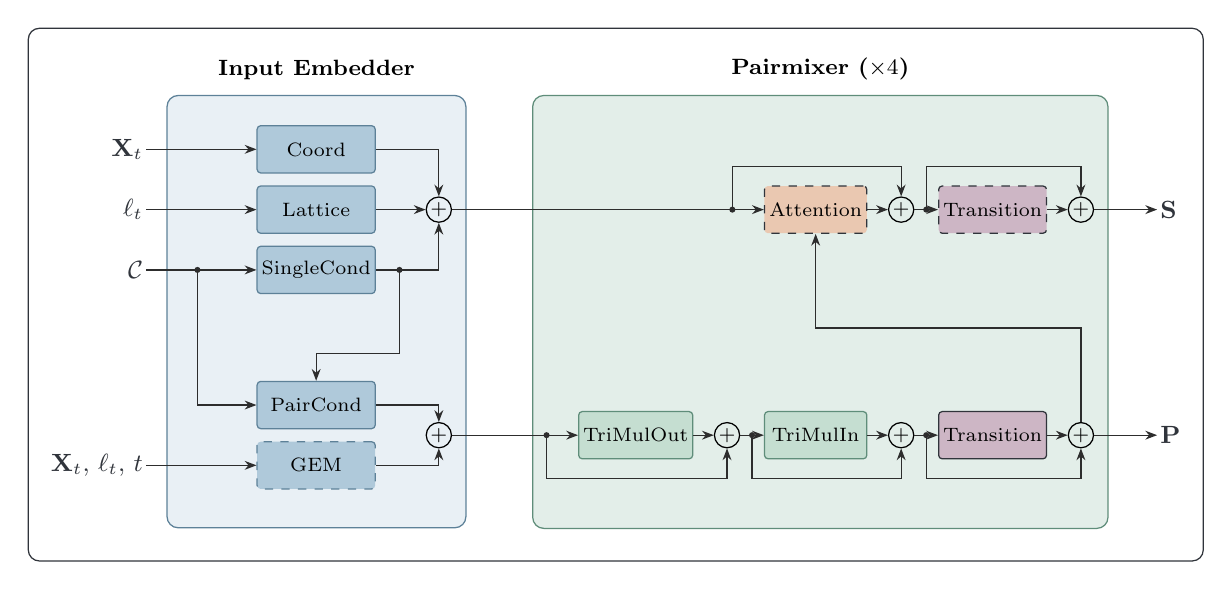
\begin{tikzpicture}[archfig]
      % Input Embedder: noisy features enter before Pairmixer
      \node[emb] (ce) {Coord};
      \node[emb, below=1.5mm of ce] (le) {Lattice};
      \node[emb, below=1.5mm of le] (sc) {SingleCond};
      \node[sum] (ssum) at ($(le.east)+(8mm,0)$) {$+$};
      \draw[fl] (ce.east) -| (ssum.north);
      \draw[fl] (le.east) -- (ssum);
      \draw[fl] (sc.east) -| (ssum.south);

      \node[emb, below=11mm of sc] (pc) {PairCond};
      \node[emb, dashed, below=1.5mm of pc] (ge) {GEM};
      \node[sum] (zsum) at ($(pc.east)!0.5!(ge.east)+(8mm,0)$) {$+$};
      \draw[fl] (pc.east) -| (zsum.north);
      \draw[fl] (ge.east) -| (zsum.south);

      \node[lab, left=14mm of ce] (inX) {$\mathbf{X}_t$};
      \node[lab, left=14mm of le] (inL) {$\boldsymbol{\ell}_t$};
      \node[lab, left=14mm of sc] (inF) {$\mathcal{C}$};
      \node[lab, left=14mm of ge] (inG)
        {$\mathbf{X}_t,\,\boldsymbol{\ell}_t,\,t$};
      \draw[fl] (inX) -- (ce.west);
      \draw[fl] (inL) -- (le.west);
      \draw[fl] (inG) -- (ge.west);
      \coordinate (condbranch) at ([xshift=-7.5mm]sc.west);
      \node[dot] at (condbranch) {};
      \draw[wire] (inF) -- (condbranch);
      \draw[fl] (condbranch) -- (sc.west);
      \draw[fl] (condbranch) |- (pc.west);
      \coordinate (cbr) at ([xshift=3mm]sc.east);
      \node[dot] at (cbr) {};
      \draw[fl] (cbr) |- ([yshift=3.5mm]pc.north) -- (pc.north);
      \coordinate (embtop) at ([yshift=2mm]ce.north);
      \coordinate (embleft) at ([xshift=-9.6mm]ce.west);
      \coordinate (modulebottom) at ([yshift=-10mm]zsum.center);
      \begin{scope}[on background layer]
        \node[modbg, draw=cEmbedDk, fill=cEmbedBg,
              fit=(embleft)(embtop)(modulebottom)(sc)(pc)(ge)(ssum)(zsum)]
              (embbg) {};
      \end{scope}
      \node[mtitle, above=0.7mm of embbg.north] (embtitle) {Input Embedder};

      % Pairmixer pair track
      \node[tri, right=16mm of zsum] (trio) {TriMulOut};
      \node[sum, right=2.6mm of trio] (za) {$+$};
      \node[tri, right=3mm of za] (trii) {TriMulIn};
      \node[sum, right=2.6mm of trii] (zb) {$+$};
      \node[trans, right=3mm of zb] (tz) {Transition};
      \node[sum, right=2.6mm of tz] (zc) {$+$};
      \draw[fl] (zsum) -- (trio.west);
      \draw[fl] (trio) -- (za);
      \draw[fl] (za) -- (trii.west);
      \draw[fl] (trii) -- (zb);
      \draw[fl] (zb) -- (tz.west);
      \draw[fl] (tz) -- (zc);
      \coordinate (rzone) at ([xshift=-4mm]trio.west);
      \coordinate (rztwo) at ([xshift=-1.5mm]trii.west);
      \coordinate (rzthree) at ([xshift=-1.5mm]tz.west);
      \foreach \point in {rzone,rztwo,rzthree} {
        \node[dot] at (\point) {};
      }
      \draw[fl] (rzone) -- ++(0,-\skipdy) -| (za.south);
      \draw[fl] (rztwo) -- ++(0,-\skipdy) -| (zb.south);
      \draw[fl] (rzthree) -- ++(0,-\skipdy) -| (zc.south);

      % Optional single-track update
      \node[attn, dashed, anchor=west] (aps) at (trii.west |- ssum) {Attention};
      \node[sum, right=2.6mm of aps] (sa) {$+$};
      \node[trans, dashed, right=3mm of sa] (tps) {Transition};
      \node[sum, right=2.6mm of tps] (sb) {$+$};
      \draw[fl] (ssum) -- (aps.west);
      \draw[fl] (aps) -- (sa);
      \draw[fl] (sa) -- (tps.west);
      \draw[fl] (tps) -- (sb);
      \coordinate (rsone) at ([xshift=-4mm]aps.west);
      \coordinate (rstwo) at ([xshift=-1.5mm]tps.west);
      \node[dot] at (rsone) {};
      \node[dot] at (rstwo) {};
      \draw[fl] (rsone) -- ++(0,\skipdy) -| (sa.north);
      \draw[fl] (rstwo) -- ++(0,\skipdy) -| (sb.north);
      \draw[fl] (zc.north) |- ($(zc.north)!0.5!(aps.south)$) -| (aps.south);
      \coordinate (pmhi) at ([yshift=\skipdy+1.5mm]aps.north);
      \coordinate (pmlo) at ([yshift=-\skipdy-1.5mm]trio.south);
      \coordinate (pairtop) at (trio |- embtop);
      \coordinate (pairbottom) at (trio |- modulebottom);
      \begin{scope}[on background layer]
        \node[modbg, draw=archPairLine, fill=cPairBg,
              fit=(rzone)(trio)(zc)(aps)(sb)(pmhi)(pmlo)(pairtop)(pairbottom)]
              (pmbg) {};
      \end{scope}
      \node[mtitle, above=0.7mm of pmbg.north] (pmtitle)
        {Pairmixer ($\times 4$)};

      % DiT inputs
      \node[lab, right=8mm of sb] (sout) {$\mathbf S$};
      \node[lab, right=8mm of zc] (pout) {$\mathbf P$};
      \draw[fl] (sb) -- (sout.west);
      \draw[fl] (zc) -- (pout.west);
      \coordinate (panelbottom) at ([yshift=-1.6mm]pmbg.south);

      \begin{scope}[on background layer]
        \node[modbg, draw=archFrame, fill=none, inner sep=7pt,
              fit=(embbg)(embtitle)(pmbg)(pmtitle)(inF)(inG)(sout)(pout)
                  (panelbottom)]
              (outerbg) {};
      \end{scope}
    \end{tikzpicture}%

  \end{minipage}\hfill
  \begin{minipage}[t]{204mm}
    \centering
    {\sffamily\bfseries\Large (b) After-Pairmixer noisy-input entry}\\[1.5mm]
    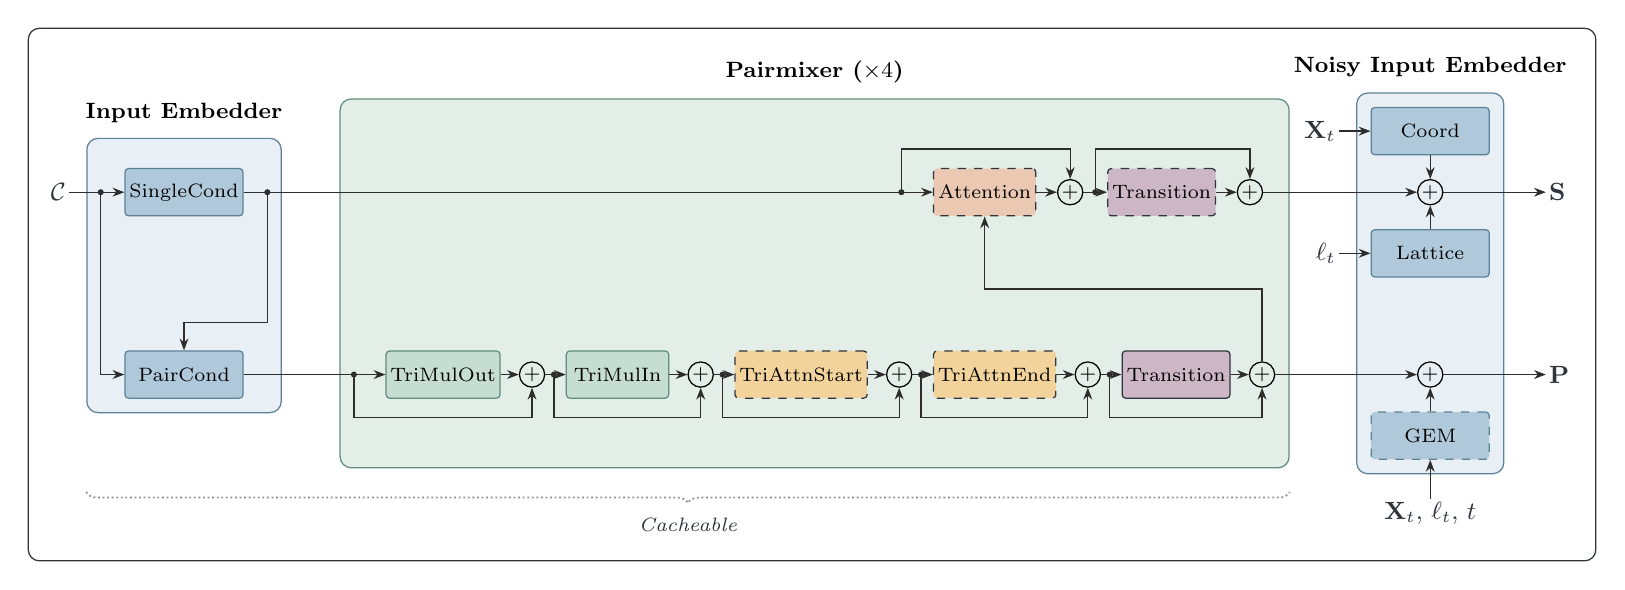
\begin{tikzpicture}[archfig]
      % Condition-only Input Embedder
      \node[emb] (sc) {SingleCond};
      \node[emb, below=17mm of sc] (pc) {PairCond};
      \node[lab, left=7mm of sc] (inF) {$\mathcal{C}$};
      \coordinate (condbranch) at ([xshift=-3mm]sc.west);
      \node[dot] at (condbranch) {};
      \draw[wire] (inF) -- (condbranch);
      \draw[fl] (condbranch) -- (sc.west);
      \draw[fl] (condbranch) |- (pc.west);
      \coordinate (cbr) at ([xshift=3mm]sc.east);
      \node[dot] at (cbr) {};
      \draw[fl] (cbr) |- ([yshift=3.5mm]pc.north) -- (pc.north);
      \coordinate (embtop) at ([yshift=2mm]sc.north);
      \coordinate (embleft) at ([xshift=-3mm]sc.west);
      \begin{scope}[on background layer]
        \node[modbg, draw=cEmbedDk, fill=cEmbedBg,
              fit=(embleft)(embtop)(sc)(pc)(cbr)] (embbg) {};
      \end{scope}
      \node[mtitle, above=0.7mm of embbg.north] (embtitle) {Input Embedder};

      % Pairmixer pair track, including optional triangle attention
      \node[tri, right=18mm of pc] (trio) {TriMulOut};
      \node[sum, right=2.3mm of trio] (za) {$+$};
      \node[tri, right=2.6mm of za] (trii) {TriMulIn};
      \node[sum, right=2.3mm of trii] (zb) {$+$};
      \node[triattn, right=2.6mm of zb] (tas) {TriAttnStart};
      \node[sum, right=2.3mm of tas] (zc) {$+$};
      \node[triattn, right=2.6mm of zc] (tae) {TriAttnEnd};
      \node[sum, right=2.3mm of tae] (zd) {$+$};
      \node[trans, right=2.6mm of zd] (tz) {Transition};
      \node[sum, right=2.3mm of tz] (ze) {$+$};
      \draw[fl] (pc.east) -- (trio.west);
      \draw[fl] (trio) -- (za);
      \draw[fl] (za) -- (trii.west);
      \draw[fl] (trii) -- (zb);
      \draw[fl] (zb) -- (tas.west);
      \draw[fl] (tas) -- (zc);
      \draw[fl] (zc) -- (tae.west);
      \draw[fl] (tae) -- (zd);
      \draw[fl] (zd) -- (tz.west);
      \draw[fl] (tz) -- (ze);
      \coordinate (rzone) at ([xshift=-4mm]trio.west);
      \coordinate (rztwo) at ([xshift=-1.5mm]trii.west);
      \coordinate (rzthree) at ([xshift=-1.5mm]tas.west);
      \coordinate (rzfour) at ([xshift=-1.5mm]tae.west);
      \coordinate (rzfive) at ([xshift=-1.5mm]tz.west);
      \foreach \point in {rzone,rztwo,rzthree,rzfour,rzfive} {
        \node[dot] at (\point) {};
      }
      \draw[fl] (rzone) -- ++(0,-\skipdy) -| (za.south);
      \draw[fl] (rztwo) -- ++(0,-\skipdy) -| (zb.south);
      \draw[fl] (rzthree) -- ++(0,-\skipdy) -| (zc.south);
      \draw[fl] (rzfour) -- ++(0,-\skipdy) -| (zd.south);
      \draw[fl] (rzfive) -- ++(0,-\skipdy) -| (ze.south);

      % Optional single-track update
      \node[attn, dashed, anchor=west] (aps) at (tae.west |- sc) {Attention};
      \node[sum, right=2.6mm of aps] (sa) {$+$};
      \node[trans, dashed, right=3mm of sa] (tps) {Transition};
      \node[sum, right=2.6mm of tps] (sb) {$+$};
      \draw[fl] (sc.east) -- (aps.west);
      \draw[fl] (aps) -- (sa);
      \draw[fl] (sa) -- (tps.west);
      \draw[fl] (tps) -- (sb);
      \coordinate (rsone) at ([xshift=-4mm]aps.west);
      \coordinate (rstwo) at ([xshift=-1.5mm]tps.west);
      \node[dot] at (rsone) {};
      \node[dot] at (rstwo) {};
      \draw[fl] (rsone) -- ++(0,\skipdy) -| (sa.north);
      \draw[fl] (rstwo) -- ++(0,\skipdy) -| (sb.north);
      \draw[fl] (ze.north) |- ($(ze.north)!0.5!(aps.south)$) -| (aps.south);
      \coordinate (pmhi) at ([yshift=\skipdy+1.5mm]aps.north);
      \coordinate (pmlo) at ([yshift=-\skipdy-1.5mm]trio.south);
      \begin{scope}[on background layer]
        \node[modbg, draw=archPairLine, fill=cPairBg,
              fit=(rzone)(trio)(ze)(aps)(sb)(pmhi)(pmlo)] (pmbg) {};
      \end{scope}
      \node[mtitle, above=0.7mm of pmbg.north] (pmtitle)
        {Pairmixer ($\times 4$)};

      % Noisy Input Embedder after Pairmixer
      \node[sum, right=18mm of ze] (zadd) {$+$};
      \node[sum] (sadd) at (zadd |- sc) {$+$};
      \node[emb, above=3mm of sadd] (ce) {Coord};
      \node[emb, below=3mm of sadd] (le) {Lattice};
      \node[emb, dashed, below=3mm of zadd] (ge) {GEM};
      \draw[fl] (sb) -- (sadd.west);
      \draw[fl] (ce.south) -- (sadd.north);
      \draw[fl] (le.north) -- (sadd.south);
      \draw[fl] (ze) -- (zadd.west);
      \draw[fl] (ge.north) -- (zadd.south);
      \node[lab, left=4mm of ce] (inX) {$\mathbf{X}_t$};
      \node[lab, left=4mm of le] (inL) {$\boldsymbol{\ell}_t$};
      \node[lab, below=5mm of ge] (inG)
        {$\mathbf{X}_t,\,\boldsymbol{\ell}_t,\,t$};
      \draw[fl] (inX) -- (ce.west);
      \draw[fl] (inL) -- (le.west);
      \draw[fl] (inG.north) -- (ge.south);
      \begin{scope}[on background layer]
        \node[modbg, draw=cEmbedDk, fill=cEmbedBg,
              fit=(ce)(le)(ge)(sadd)(zadd)] (noisybg) {};
      \end{scope}
      \node[mtitle, above=0.7mm of noisybg.north] (noisytitle)
        {Noisy Input Embedder};

      % DiT inputs
      \node[lab, right=13mm of sadd] (sout) {$\mathbf S$};
      \node[lab, right=13mm of zadd] (pout) {$\mathbf P$};
      \draw[fl] (sadd) -- (sout.west);
      \draw[fl] (zadd) -- (pout.west);

      % Condition-only computation can be reused across denoising steps
      \coordinate (cachebraceleft) at (embbg.west |- pmbg.south);
      \coordinate (cachebraceright) at (pmbg.east |- pmbg.south);
      \draw[draw=archFrame!55, line width=0.65pt, densely dotted, decorate,
            decoration={brace, mirror, amplitude=4pt}]
        ([yshift=-3mm]cachebraceleft) -- ([yshift=-3mm]cachebraceright)
        node[midway, below=2mm, font=\scriptsize\itshape, text=archFrame]
        (cachelabel) {Cacheable};

      \begin{scope}[on background layer]
        \node[modbg, draw=archFrame, fill=none, inner sep=7pt,
              fit=(embbg)(embtitle)(pmbg)(pmtitle)(noisybg)(noisytitle)
                  (inF)(inG)(sout)(pout)(cachelabel)] (outerbg) {};
      \end{scope}
    \end{tikzpicture}%
  \end{minipage}
  \end{minipage}
  }
    \caption{\textbf{Model variants for architecture ablations.}
    \textbf{(a)} In the pre-entry variant, noisy coordinate and lattice embeddings
    and optional geometric enhancement module (GEM) features are injected before
    \textsc{Pairmixer}. \textbf{(b)} In the post-entry variant, the condition-only
    \textsc{Input Embedder} and \textsc{Pairmixer} are evaluated before noisy-state
    injection, allowing their outputs to be cached across denoising steps. Modules
    with dotted outlines denote optional components. Both variants produce single
    and pair representations $\mathbf S$ and $\mathbf P$, which are passed to the
    same DiT trunk.}
  \label{fig:sp-architecture}
\end{figure}
